\chapter{LHC and CMS experiment}

Large Hadron Collider~\cite{LHC_refer} is the most powerful hadron collider ever built. The circumference of this circle superconducting collider is 26.7 km and the designed full operation energy is 14 TeV. In 2012 LHC operates on 8 TeV and in 2016, it boosts up to 13 TeV. There are four experiments hold on the LHC ring, ALICE, ATLAS, CMS and LHCb. ATLAS and CMS are general purpose detectors, aiming for the high luminosity in the order $L=10^{34} cm^{-2}s^{-1}$. LHCb focuses on the b physics study, while ALICE studies the lead-lead collision.

\section{LHC accelerator}

A sketch view of the proton accelerating process is shown in Figure.~\ref{fig:LHC_sketch}. LHC is the last and most powerful accelerator in the accelerating chain. Before the beams are injected into LHC, a series of steps are taken. For the proton-proton(p-p) collision, protons are from the source Duoplasmatron, which uses electric field to break down hydrogen gas into protons and electrons, then protons are accelerated by a 90 kV supply. Leaving the source, the protons are focused and accelerated to 750 keV by radio frequency quadrupole. Then the protons are further accelerated by linear accelerator Linac2 to 50 MeV. Proton synchrotron booster further accelerate protons from 50 MeV to 1.4 GeV and injects protons into Proton synchrotron(PS). PS accelerates protons to 25 GeV followed by the super proton synchrotron which boost the protons to 450 GeV. LHC is the last ring in the whole accelerating process and accelerate the protons to its final energy 6.5 GeV(or 7 GeV). In a normal fill with protons, LHC holds 2808 bunches with an approximation of $10^{11}$ protons.

There are thousands of superconducting magnets along the LHC ring to bend and focus the beam. Among the magnets, there are 1232 main dipoles, which are used to bend the beam with an operating field above 8 T. Other types of magnets, for example, quadrupoles magnets can tight the beam either vertically or horizontally while  sextupole, octupole and decapole can help fine tuning the magnetic field. The radiofrequency cavities(RF) in the LHC are used to accelerate the protons from 450 GeV to 6.5 GeV(or 7 GeV), keep the bunches in the beam pipe compact and store the energy loss from synchrotron radiation. Eight RFs per beam, providing 16 MV  longitudinal oscillating voltage with the 400 MHz superconducting cavity system. 

Machine luminosity is an important parameter of the collider. For a process under study, the number of events created per-second $N_{\textrm{event}}$ is shown in Equation.~\ref{event_number}, in which L is the machine luminosity and $\sigma_{event}$ is the cross section of that process.

\begin{align}\label{event_number}
N_{\textrm{event}}=L\sigma_{event}
\end{align}

Machine luminosity is determined by a number of factors as shown in Equation.~\ref{Lumi_express}. $n_b$ and $N_{b}$ are the number of bunches per-beam and the number of protons per-bunch.$f_{rev}$ and $\gamma_{\gamma}$ are the revolution frequency and relativistic gamma factor respectively. $\beta*$ is the amplitude function of the beam at the collision point while function F describes the reduction of luminosity because of the crossing angle. This machine luminosity is also called instantaneous luminosity which is the luminosity at a unite time. The integrated luminosity which later referred as luminosity is instantaneous luminosity integrating over time~\ref{fig:LHC_sketch}.  

\begin{align}\label{Lumi_express}
L=\frac{N_{b}^{2}n_{b}f_{fev}\gamma_{\gamma}}{4\pi\epsilon\beta*}F
\end{align}



\begin{figure}[htbp] 
\centering
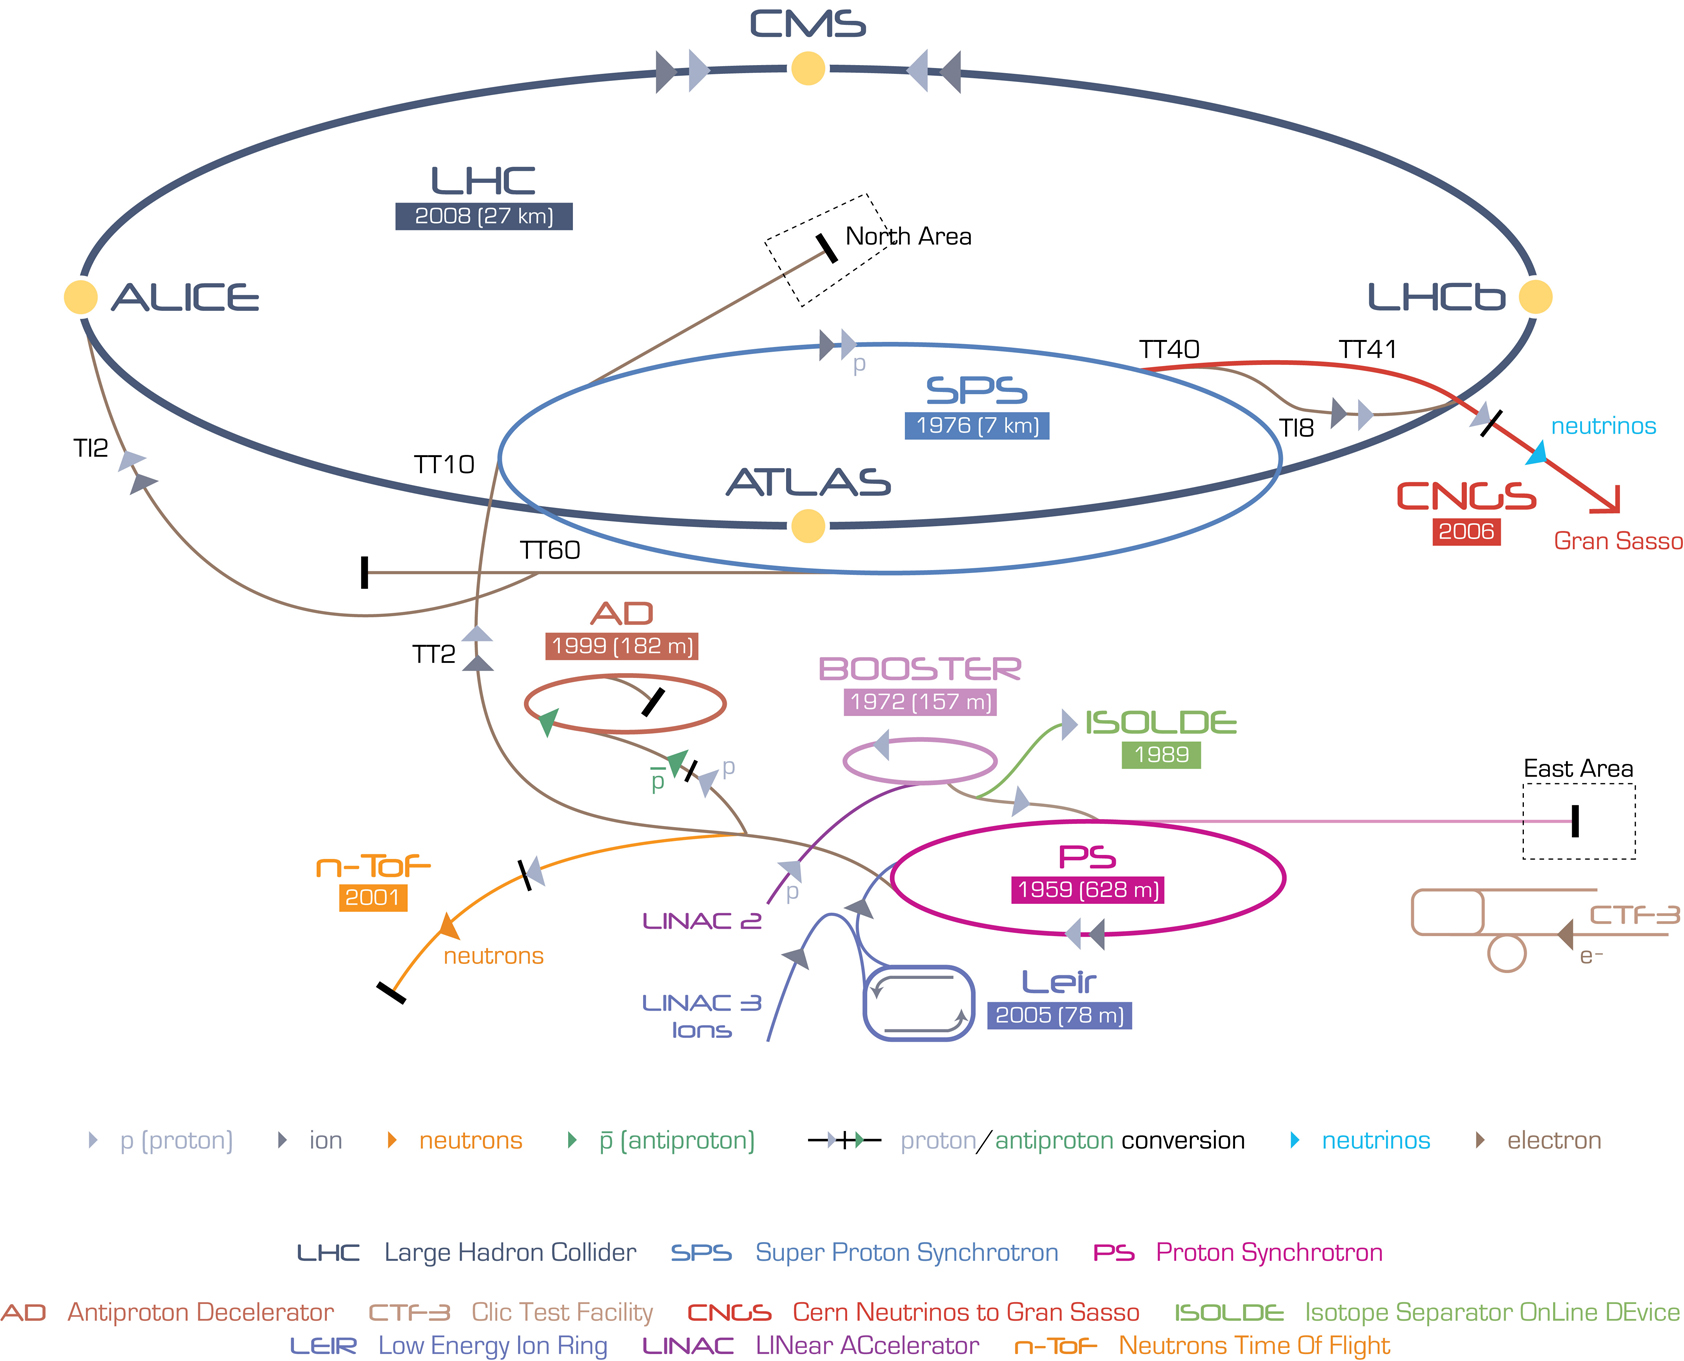
\includegraphics[width=0.8\textwidth]{chapter3/LHC_chain.jpg}
\caption{A sketch view LHC injection chain and main experiments associated~\cite{Christiane:1260465}.}
\label{fig:LHC_sketch}
\end{figure}


\section{Compact Muon Solenoid}
Compact muon solenoid(CMS) is a general purpose detector, which institutes in one of LHC collision point. It is a high performance detector that covers a broad range of physics researches, like Standard model physics, supersymmetry and dark matter. CMS detector is designed to have good muon momentum and position resolution over large range of energy and angles, good charged particle momentum resolution and high identification efficiency within inner tracker, good electromagnetic energy and position resolution and high photon and lepton isolation efficiency in high luminosity condition, good missing transverse momentum and jet energy resolution.  


An general view of CMS detector is shown in Figure.~\ref{fig:CMS_sketch}. The detector is composed of a set of sub-detectors from the inside and out in a ring structure. The main sub-detectors are the following:

\begin{figure}[htbp] 
\centering
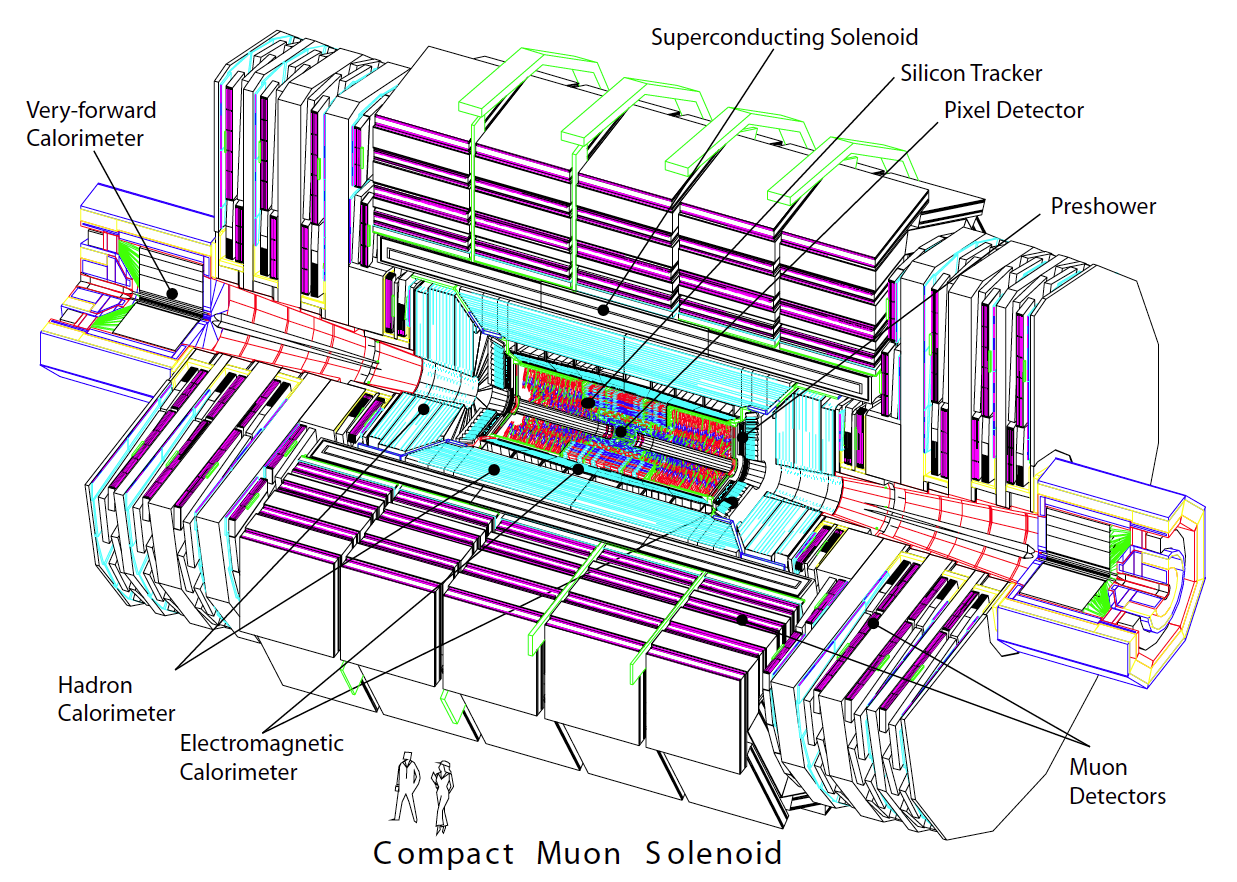
\includegraphics[width=0.8\textwidth]{chapter3/CMS_detecter.png}
\caption{A sketch view of CMS detector~\cite{CMS_experiment}}
\label{fig:CMS_sketch}
\end{figure}


\begin{enumerate}[$\bullet$]
\item Tracker consists two parts, the pixel detector and silicon tracks which are used measure the momentum and tracks of the charged particles.
\item Electromagnetic calorimeter mainly measures the energy and the position of electrons and photons. Other particles will leave some percentage of energy inside. 
\item Hadron calorimeter measures the energy of hadrons 
\item Muon detector measures the tracks and momentum of the muons.
\end{enumerate} 

Another outstanding feature of CMS is the superconducting magnet system, which provide a 3.8 T magnetic field. The configuration of the magnet system drives the design and layout of the detector. Besides the sub-detectors listed above, trigger system is also crucial for the success of the whole program. Trigger system consists two parts, the hardware based level one trigger and the software based high level trigger. Trigger system does the initial selection of interesting events from a huge flux of events per-collision, which makes it possible for data-acquisition and recording. The details of the sub-detectors and other systems mentioned will be presented later. 

In general CMS detector is 21.6 m long, 14.6 in diameter and weighted 12500 tonnes in total. The coordinate system adopted by CMS sets the center at the collision point. The x-axis points towards the center of LHC and z-axis points along the beam direction. The azimuthal angle $\phi$ is used to measure the angle from x-axis in the x-y plane and polar angle $\theta$ measures the angle from z-axis and r is the radial coordinate. Another variable called the pseudorapidity $\eta$, defined as $\eta=-\textrm{ln}\textrm{tan}(\theta/2)$ is also frequently used in the measurements. In the case $E\gg m$, pseudorapidity can be approximated as $\eta=-\textrm{ln}\big(\frac{E+p_{z}}{E-p_{z}}\big)$, where $p_{z}$ is the longitudinal component of momentum~\cite{CMS_experiment}. 

\subsection{Tracker}
The main purpose of inner tracking system of CMS is measuring the trajectories of charged particles from the LHC collision. The efficient and precise measurement is crucial for the reconstruction and identification of particles. LHC operates with the instantaneous luminosity in the order of $10^{34}cm^{-2}s^{-1}$, in average more than 20 p-p interactions and 1000 particles per-bunch crossing. High granularity and fast response is primary important for the tracker system. To measure the trajectories precisely, low interaction of tracker materials with incoming particles, like multi-scattering, photon conversion and nuclear interaction is also important. In the long operation period, radiation hardness of the tracker material is needed. All of these factors drive the design of CMS tracker system.

The tracker system of CMS surrounds the collision point with the dimension 5.8 m in length and 2.5 m in diameter, with a coverage up to pseudorapidity $|\eta|<2.5$. A overview of the tracker system layout is shown in Figure.~\ref{fig:tracker_sketch}. Three layers of silicon pixel detector modules surround the interaction points and two additional disks of pixel modules on each side, in all 66 million pixels of the size $100\times150 \mu m$ each. Following the pixel detector is the silicon strip tracker. There are four components of strip tracker, tracker Inner barrel(TIB), tracker inner Discs(TID), tracker outer barrel(TOB) and tracker end caps(TEC). The strip tracker components arrangement as shown in Figure.~\ref{fig:tracker_sketch}, consisting of about 10 million strips and 10 layers. 


\begin{figure}[htbp] 
\centering
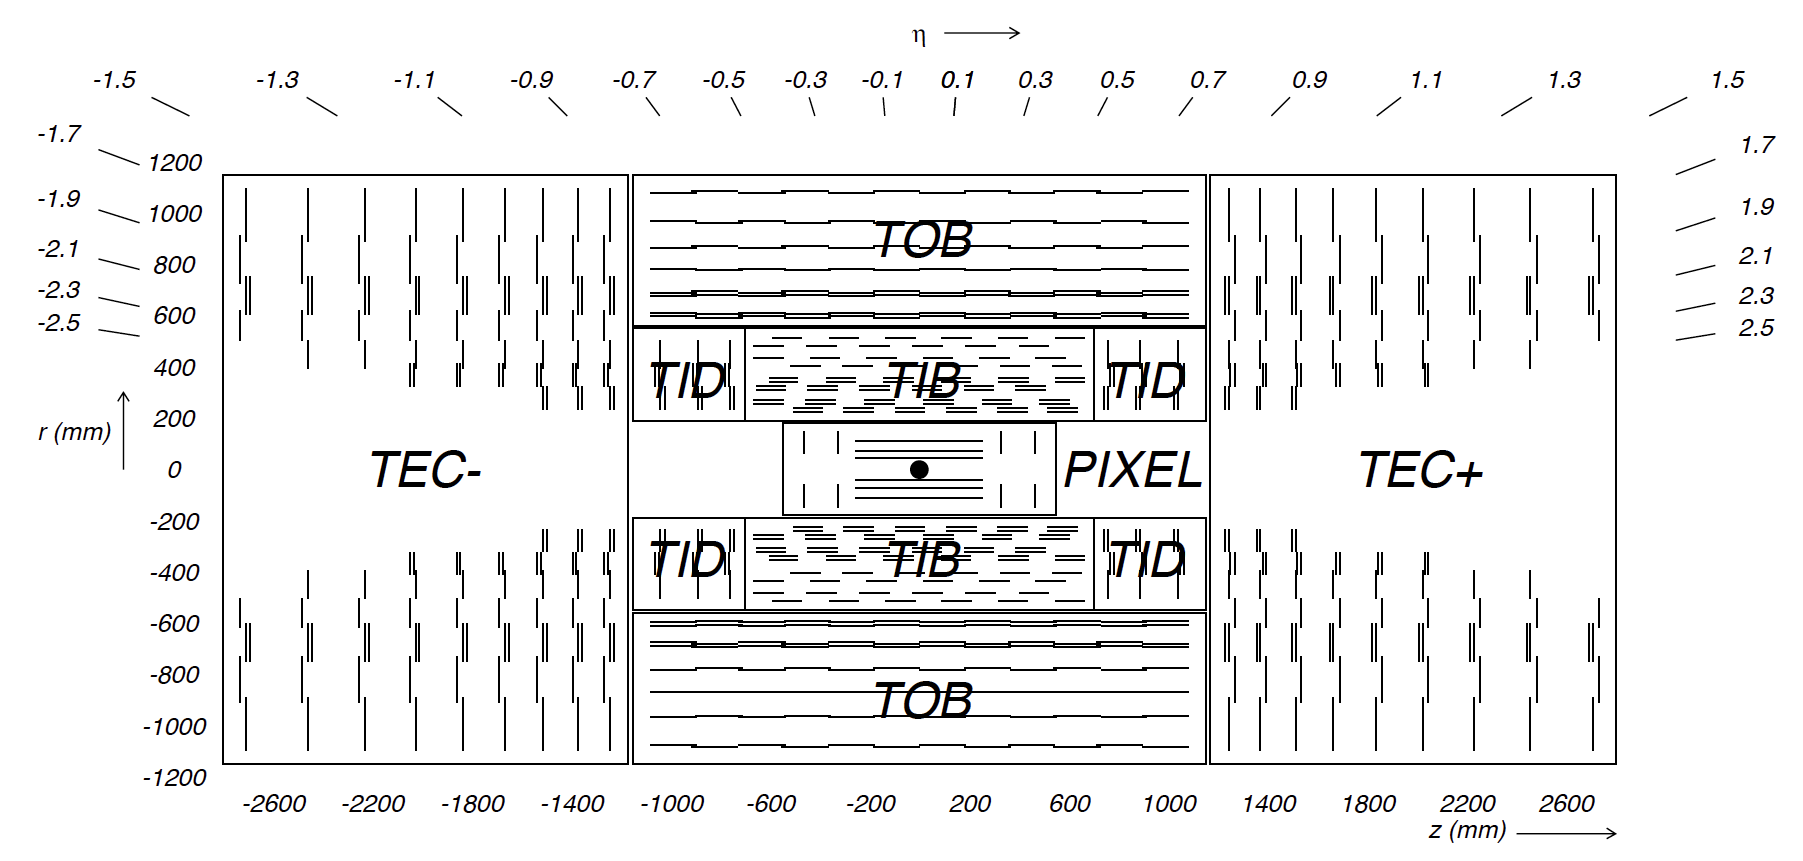
\includegraphics[width=0.8\textwidth]{chapter3/Tracker_structure.png}
\caption{The structure of tracker in CMS~\cite{CMS_experiment}}
\label{fig:tracker_sketch}
\end{figure}



\subsection{The electromagnetic calorimeter}

The CMS Electromagnetic calorimeter(ECAL) is a hermetic homogeneous lead tungstate($PbWO_{4}$) calorimeter. The whole sub-detector is composed of two parts, the central barrel(EB) covering the range $|\eta|<1.479$ and the endcap disks(EE) covering the range $1.479<|\eta|<3.0$. EB is made up of 61200 $PbWO_{4}$ crystals with $22\times22~mm^{2}$ in the front face, 23 cm in length(25.8 in radiation lengths). EE is made up of 7324 crystals per disk with front face $29\times29~mm^{2}$, 22 in length(24.7 in radiation lengths) and a preshower detector(ES)~\cite{CMS_TDR}. The geometrical configuration of ECAL is shown in Figure.~\ref{fig:ECAL_sketch}. 

The $PbWO_{4}$ crystals used in ECAL have high density(8.28 $g/cm^{3}$), short radiation length(0.89 cm) and small Moli$\grave{e}$re radius(2.2 cm), together with the specific geometrical parameters used, rendering ECAL  good energy resolution, fast response, fine granularity and radiation resistant. Photodetectors are placed at the end of the crystals. In EB, avalanche photodiodes(APDs) are used, while vacuum phototriodes(VPTs) are used in EE. Both types of the photodiode show good performance in the environment with hard radiation and 4-T magnetic field. ES is in front of EE in the pseudorapidity range $1.653<|\eta|<2.6$. ES is a sampling detector with silicon strip sensors placed behind the lead radiator to measure the energy and position of the incoming particles.  

\begin{figure}[htbp] 
\centering
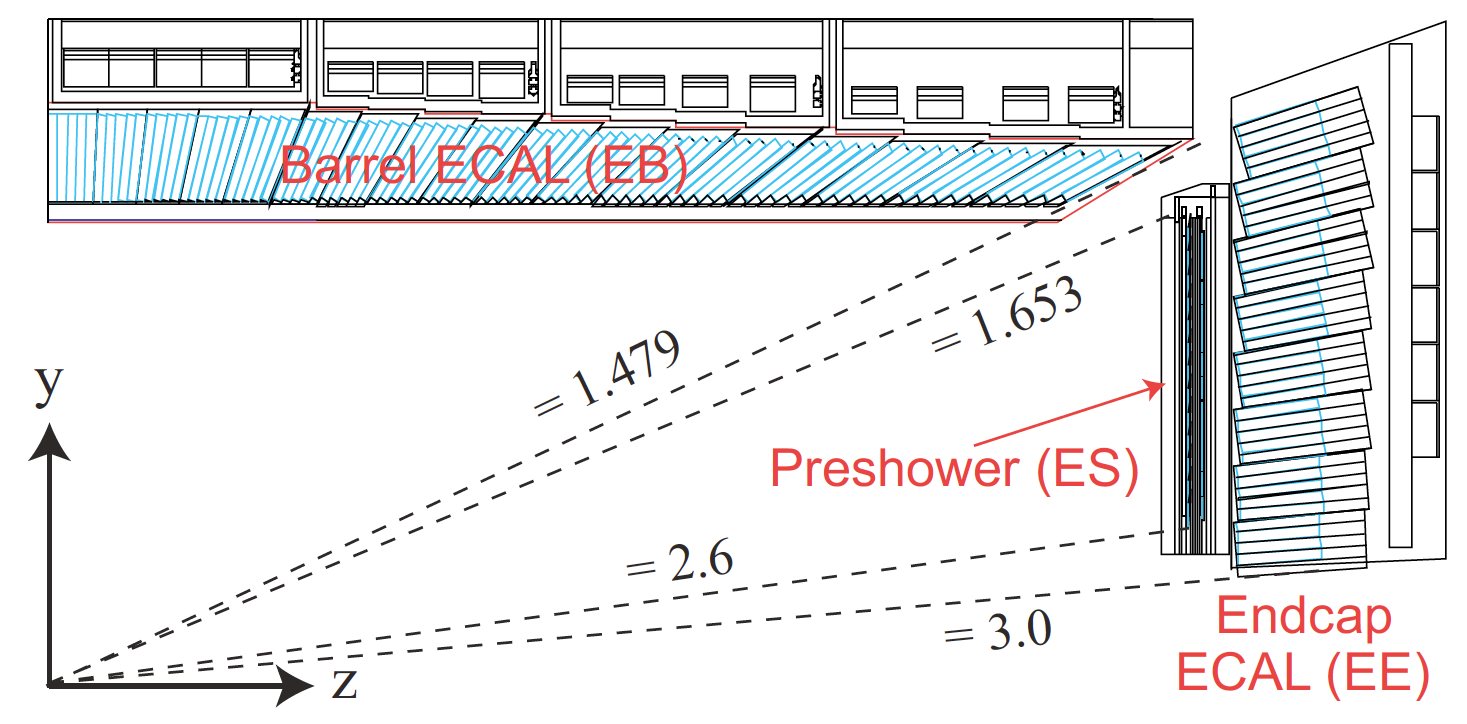
\includegraphics[width=0.8\textwidth]{chapter3/ECAL_transverse.png}
\caption{ECAL geometrical configuration~\cite{CMS_TDR}}
\label{fig:ECAL_sketch}
\end{figure}

Each half of EB is composed of 18 supermodules that one contains 1700 crystals. The $PbWO_{4}$ crystal relative energy resolution is measured with ECAL supermdules directly exposed to electron beam without considering the materials in front as the case in reality. The relative energy resolution as a function of electron energy can be expressed as 
%spikes
% np scattering in the protective epoxy coating of the APD, and the resulting proton directly ionizing the APD active volume.
\begin{align*}
\frac{\sigma}{E}=\frac{2.8\%}{\sqrt{E/\textrm{GeV}}}\oplus\frac{12\%}{E/\textrm{GeV}}\oplus 0.3\%
\end{align*}

The first term stands for the contribution from stochastic factors, like the number fluctuation in production of the secondary particles. The second term is the noise contribution coming from electronics and digitization, while the last is a constant term that covers the other factors~\cite{ECAL_EB_reso}.

\subsection{The hadron calorimeter}

CMS hadron calorimeter(HCAL) is a hermetic sampling calorimeter, which is important for the measurement of the energy and momentum of hadrons, also the missing energy that caused by the non-interacting particles.  HCAL is composed mainly by HCAL barrel(HB), HCAL endcaps(HE) and forward calorimeter(HF). The mechanical structure of HCAL is shown in Figure.~\ref{fig:HCALL_sketch}. 

\begin{figure}[htbp] 
\centering
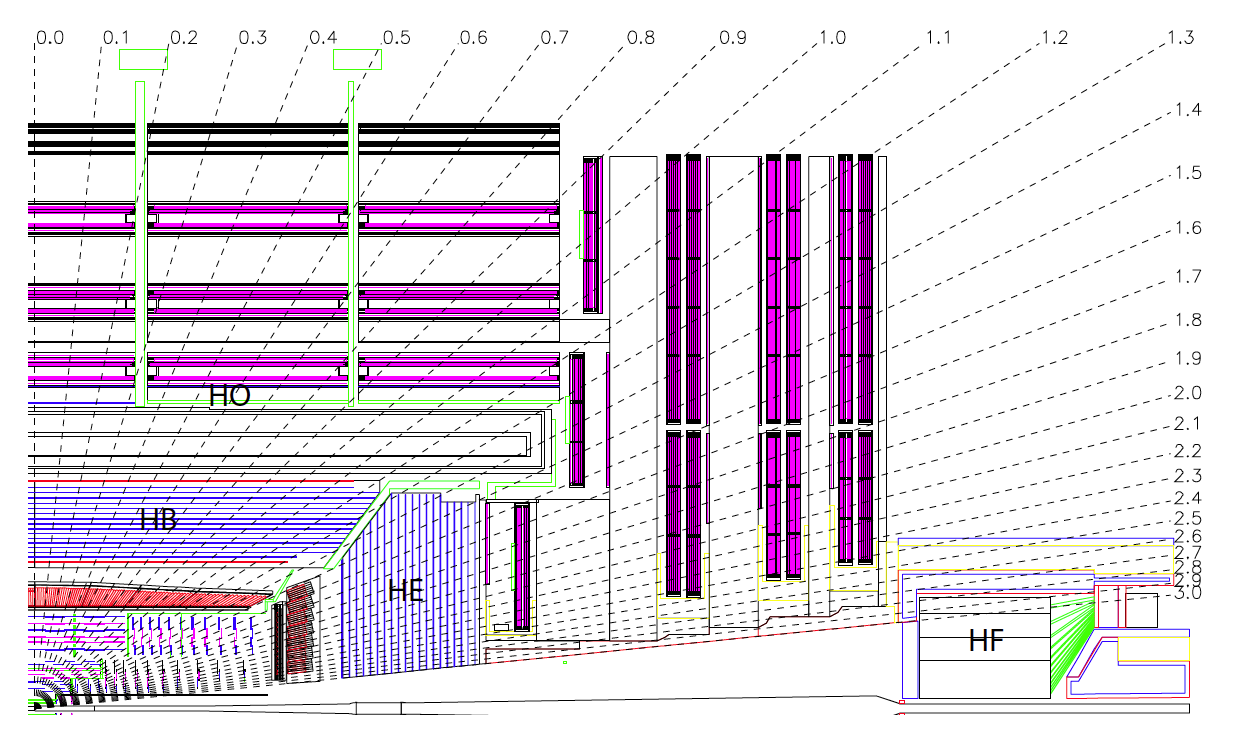
\includegraphics[width=0.8\textwidth]{chapter3/HCAL_sketch.png}
\caption{A longitudinal view of CMS HCAL sub-detector~\cite{CMS_experiment}}
\label{fig:HCALL_sketch}
\end{figure}


HB is mostly composed of  several layer of brass absorber plates, between which are the plastic scintillator tiles. The inner most and out most layer plates are made of stainless steel to gain structural strength. When hadrons hit the absorber, secondary particles are produced in showers. As the showers develops, the alternating layers of scintillators are activated and emit blue-violet light. The lights are collected as signals. HB covers the central pseudorapidity range $|\eta|<1.3$ with a individual read out unit $\Delta \eta\times\Delta\phi=0.087\times 0.087$. To have enough sampling depth in HCAL central region because of the limited spaces between ECAL and muon detector, an extra outer calorimeter(HO) is installed.  HO utilizes the outside solenoid coil as additional absorber to insert plastic scintillators. Similar to HB, HE is also made of brass absorber and plastic scintillator tiles layers, which covers the range $1.3<|\eta|<3.0$. The read out units has the geometry $\Delta \eta\times\Delta\phi=0.17\times 0.17$ in HE~\cite{CMS_experiment}. An combined ECAL and HCAL energy resolution~\cite{HCAL_reso} measured in test beam with pions is 

\begin{align*}
\frac{\sigma}{E}=\frac{110\%}{\sqrt{E/\textrm{GeV}}}\oplus 0.9\%
\end{align*}

HF situates $\pm11$ m from the interaction point to complement the large pseudorapidity measurement of HE in the range $3.0<|\eta|<5.0$. HF is made of grooved steel plates with quartz fibers. Charged shower particles generate Cherenkov light, which is collected by the quartz fibers as signals. Radiation hardness is critical for the operation of HF.   



\subsection{Muon detector}
CMS muon detector is designed to measure the momentum and charge of muons. Three types of gas detectors are used in CMS, the   barrel drift tube(DT) chambers, the cathode strip chambers(CSC) in the endcaps and resistive plate chambers(RPC) in both barrel and endcap regions. 

In muon detector barrel(MB), DT chambers and RPCs are used which covers the pseudorapidity region $|\eta|<1.2$. MB is composed of 250 chambers. The chambers are located in 4 stations inside the magnet return yoke. The yoke is further divided into 5 wheels, each of which is composed of 12 sectors. As shown in Figure.~\ref{fig:muon_sketch}, the stations are named MB1 to MB4, which are composted one DT chamber and varied number of RPCs that depending one the exact location. DT chamber measures the position the incoming muon which knocks off electrons of the gas atoms in the chamber and collected by a large numbers of charged wires inside.% The gas used in DT chambers is a mixture of Ar and $\textrm{CO}_{2}$.

In muon detector endcaps(ME), 468 CSCs which covers the range $0.9<|\eta|<2.4$ are used. ME also composed of 4 stations of chambers and in each of the discs. CSC is in a wedge shape and composed of 6 gas gaps. The gap is filled in with a cathodes strip and anode wires what running perpendicularly to the strip. When a muon comes, the knocked off electrons creating avalanche and received by the positive charged wires.  

Both DT chambers and CSCs measure the position and can also trigger on the $\pt$ of muons. To better deal with the high luminosity and improving the trigger muon $\pt$ resolution, the dedicated trigger system RPCs are added to both MB and ME. RPC is a double-gap bakelite chamber which operates with the avalanches that caused by the muons. RPC can provide additional fast triggering and sharp $\pt$ threshold. Four RPCs layers are used in the MB first two stations(two each) and another two layers(one each) are used in the last two stations.  In the ME, one RPC layers in each of the first three stations.    



\begin{figure}[htbp] 
\centering
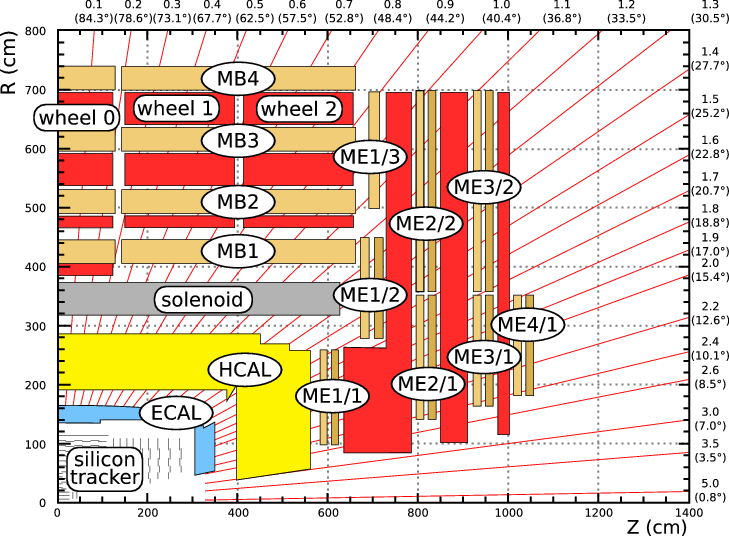
\includegraphics[width=0.8\textwidth]{chapter3/Muon_chambers.png}
\caption{A overview of muon chamber configuration in CMS~\cite{Muon_chambers}}
\label{fig:muon_sketch}
\end{figure}


\subsection{Trigger}

LHC is a high luminosity collider in the order of $10^{34}\textrm{cm}^{2}\textrm{s}^{-1}$. In the p-p collision, the bunch crossing time is 25 ns and the corresponding frequency is 40 MHz. In each of the 25 ns, there are approximately 20 collisions. This high rate makes it impossible to transmit and record all of the events, also it is not necessary, since most of the events are not of current physics research interests. CMS use a two level trigger system to select events and reduce the event recording rate, Level-1(L1) trigger and High-level trigger(HLT) systems. 


L1 trigger is based on custom designed and programmable electronics, situated inside the detector. It utilizes the information from calorimeters and muon system, performing simplified but effective reconstructions, corrections and selections, which reduces the event rate from 40 MHz to 100 kHz. In LHC Run II, the L1 trigger system has been upgraded to deal with the increased luminosity and improve the performance. The L1 calorimeter trigger accesses the information from the whole ECAL and HCAL in the granularity of trigger tower level, which approximately correspond to a region $0.087\times0.087$ in $\eta$ and $\phi$. The trigger reconstructs the $\Pe/\gamma$, jets, $\tau$ and the sum energy of the candidates with the algorithms implemented in the time multiplexed trigger architecture~\cite{TMT_trigger}. The algorithms implemented at hardware trigger level, with dynamic clustering of trigger towers, pile-up migration and innovated tau and jet reconstruction with various look-up table for the calibrations and corrections~\cite{L1_Egamma}. The L1 muon trigger system fully utilizes three muon detectors in the track reconstruction. In general, the track reconstruction of muons are divided into three regions, barrel, overlap and endcap, based on the geometry. Through dedicated construction algorithm, the tracks are built, so as computing the muon qualities. There informations are used in the triggering processes~\cite{L1muontrigger}. 


HLT in CMS further reduced the event rate from 100 kHz(after L1 trigger selection) down to 1 kHz that is a possible rate for event storage. HLT is software based trigger system and utilized the streamlined version of the CMS soft-ware for event reconstruction on the large computer farm~\cite{CMS_trigger_RUNII}. Maximizing the trigger efficiency and keeping acceptable CPU-time is crucial. HLC accesses to the full granularity and sub-detectors of CMS, including the tracker. The dedicated algorithms used in HLT is the very closed to the ones used in the off-line reconstruction and analysis, besides the for some different parameter configurations~\cite{CMS_HLT_RunII}.             








%\subsubsection{Level 1 Trigger}
%probably I have to put something there2



%\subsubsection{High Level Trigger}

